\chapter{Rencana Umum Proyek}
\label{app:rencana-umum}

Proyek Tugas Akhir Capstone ini merupakan proyek pengembangan sistem \emph{chatbot} asisten hukum berbasis \emph{Retrieval-Augmented Generation} (RAG), \emph{Knowledge Graph}, dan \emph{Explainable Artificial Intelligence} (XAI) untuk mendukung pencarian dan pemahaman peraturan perundang-undangan Indonesia di bidang pendidikan. Sistem ini dirancang sebagai sebuah aplikasi dengan antarmuka yang digunakan oleh seluruh pengguna.

Pengguna berinteraksi dengan sistem melalui antarmuka \emph{chatbot} untuk mengajukan pertanyaan hukum sebagai \emph{user query}. Sistem kemudian memproses pertanyaan tersebut dengan memanfaatkan basis data peraturan yang telah melalui proses \emph{Data Processing Orchestrator} (DPO), \emph{Retrieval-Augmented Generation} (RAG), dan \emph{Explainable Artificial Intelligence} (XAI) sebelum akhirnya menghasilkan respons berupa jawaban hukum yang disertai penjelasan dan dasar hukum yang relevan.

Gambar~\ref{fig:system-overview} menunjukkan diagram posisi dan alur interaksi sistem \emph{chatbot} hukum yang akan dikembangkan.

\begin{figure}[H]
    \centering
    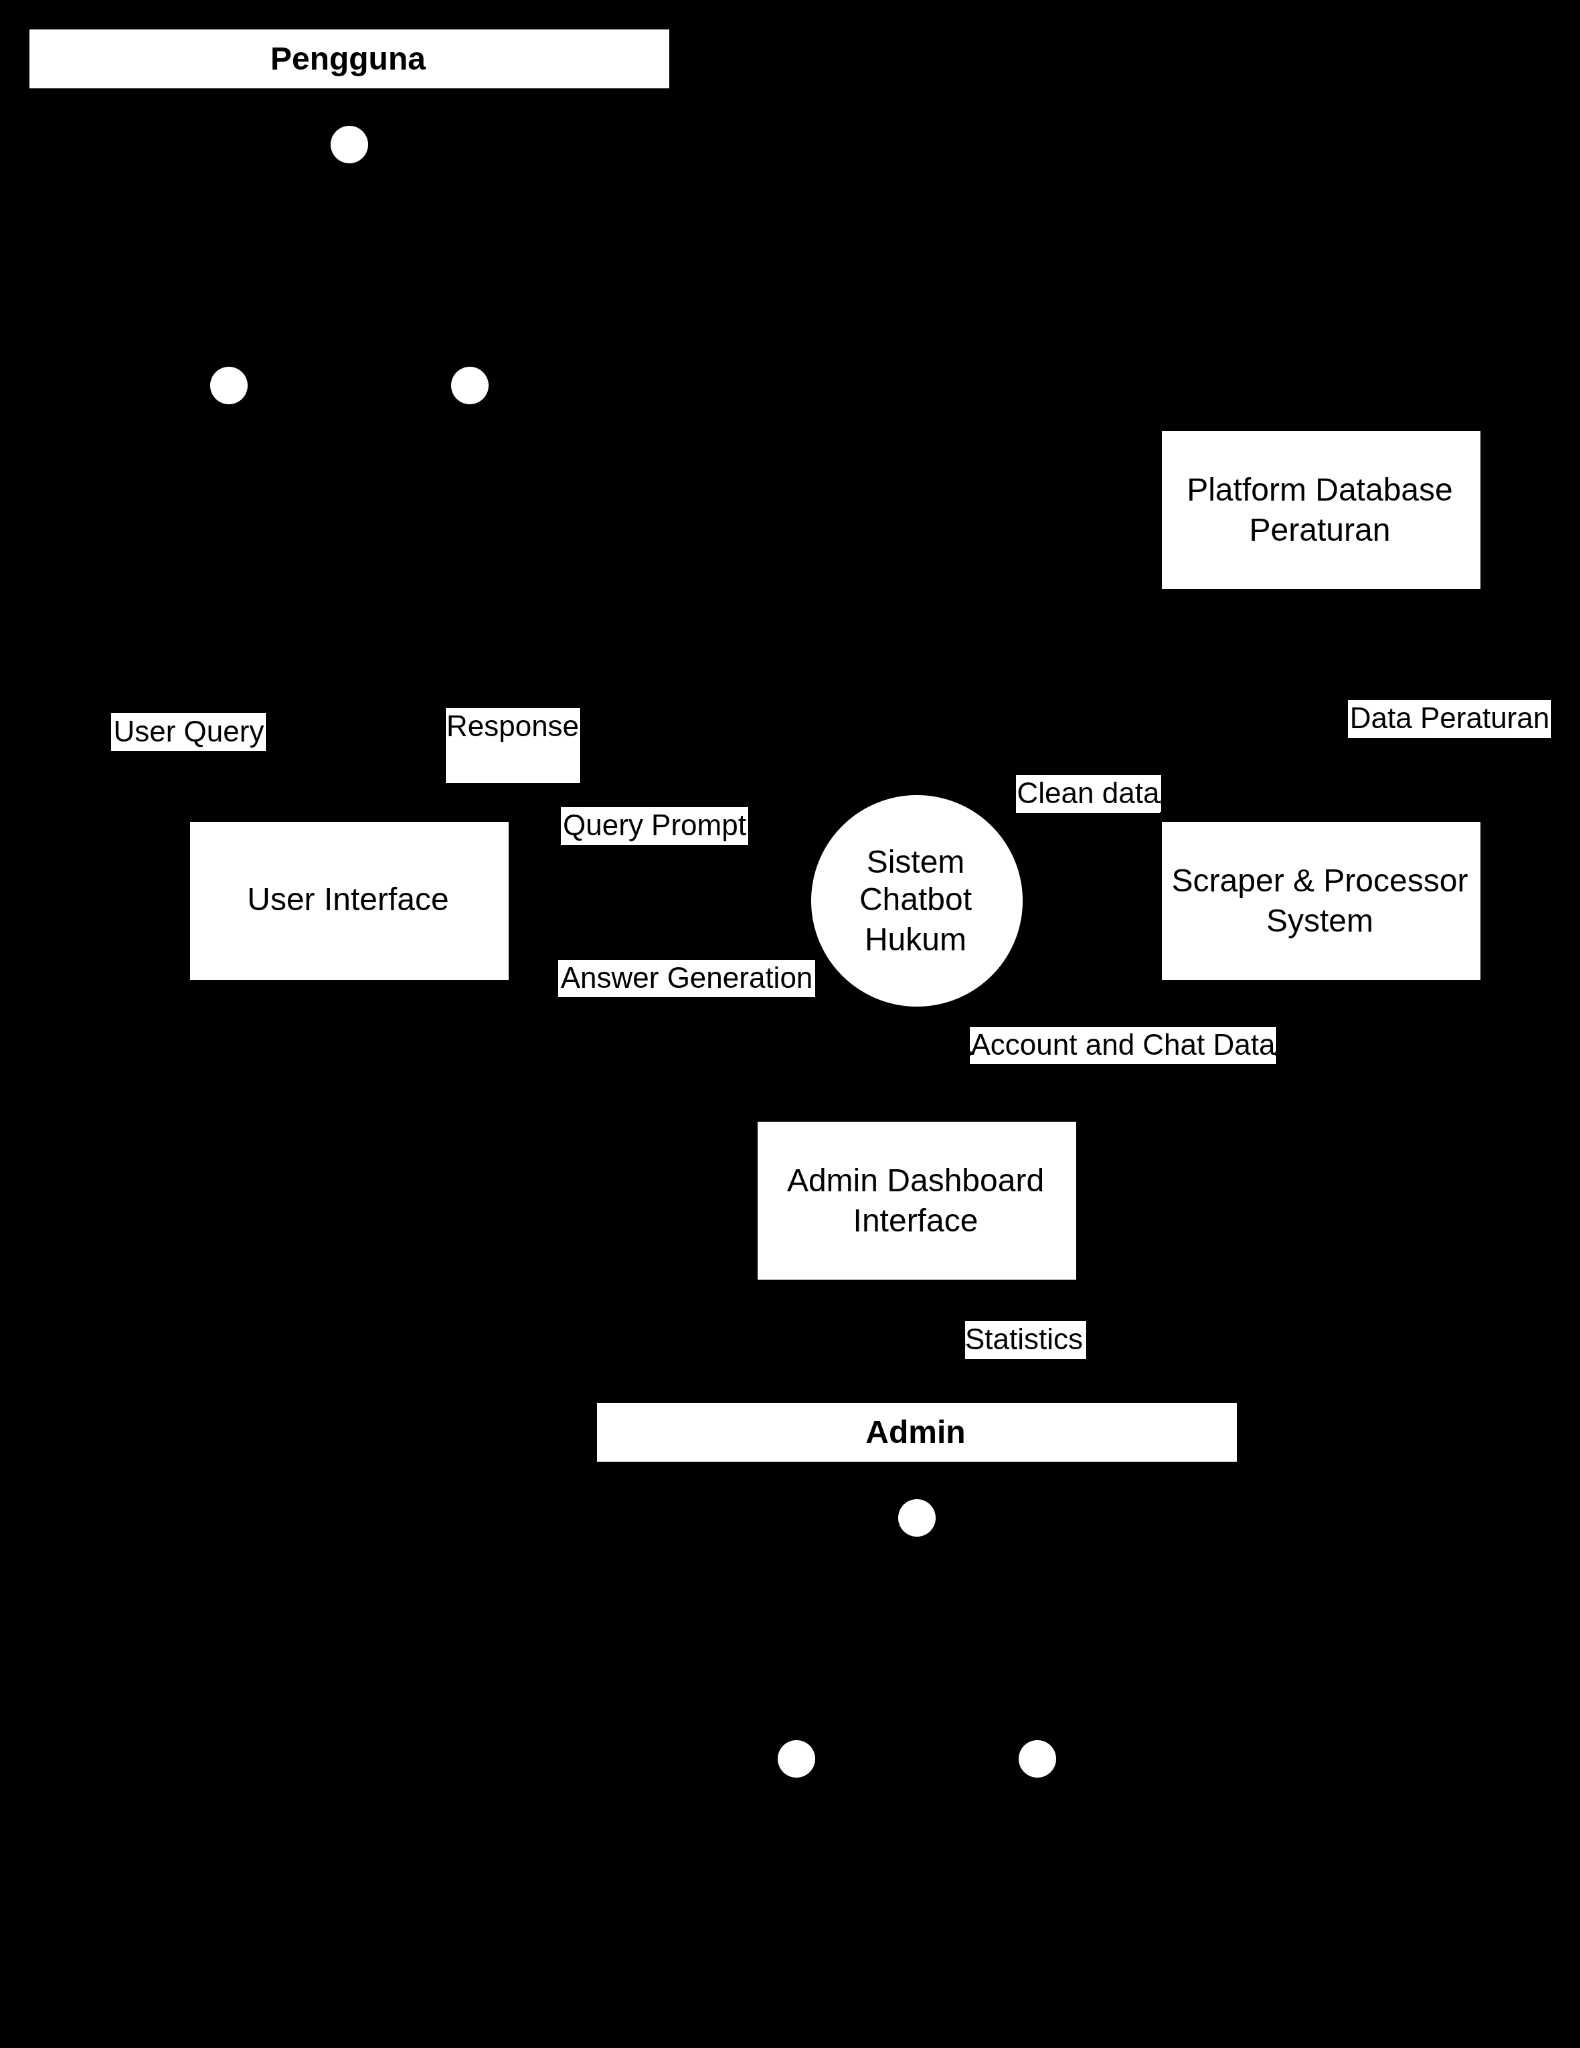
\includegraphics[width=0.82\textwidth]{images/reference-013.png}
    \caption{Diagram Sistem \emph{Chatbot} Hukum.}
    \label{fig:system-overview}
\end{figure}

Berdasarkan diagram tersebut, sistem \emph{chatbot} hukum terdiri atas beberapa komponen yang dapat dilihat pada Tabel~\ref{tab:entities}.

\begin{table}[H]
\centering
\caption{Deskripsi Entitas pada Sistem \emph{Chatbot} Hukum}
\label{tab:entities}
\small
\begin{tabularx}{\textwidth}{|p{0.25\textwidth}|X|}
\hline
\textbf{Entitas} & \textbf{Deskripsi} \\
\hline
Pengguna & Pengguna merupakan entitas yang mengajukan pertanyaan hukum kepada sistem \emph{chatbot}. Seluruh pengguna dapat berinteraksi melalui \emph{user query}. \\
\hline
\emph{User Interface} & \emph{User Interface} berfungsi sebagai media interaksi antara pengguna dan sistem \emph{chatbot} hukum. Melalui antarmuka ini, pengguna memasukkan \emph{user query} dan menerima \emph{response} berupa jawaban hukum yang dihasilkan oleh sistem. \\
\hline
Sistem \emph{Chatbot} Hukum & Sistem \emph{Chatbot} Hukum merupakan komponen inti yang memproses \emph{query} dari pengguna. Sistem ini bertanggung jawab atas pemrosesan, \emph{retrieval} konteks hukum dari basis data, \emph{reasoning} berbasis \emph{legal knowledge graph}, serta generasi jawaban dengan mekanisme \emph{explainable artificial intelligence}. \\
\hline
\emph{Scraper \& Processor System} & Komponen ini bertugas melakukan pengambilan data peraturan perundang-undangan dari sumber resmi, kemudian melakukan proses \emph{cleaning}, \emph{formatting}, dan pemrosesan struktur dokumen hukum. Hasil pemrosesan berupa data peraturan yang bersih dan terstruktur digunakan sebagai basis pengetahuan sistem \emph{chatbot}. \\
\hline
Platform \emph{Database} Peraturan & Platform \emph{database} peraturan berfungsi sebagai sumber terpusat untuk data peraturan perundang-undangan. \\
\hline
\end{tabularx}
\end{table}

Selama proses pengembangannya, sistem \emph{chatbot} hukum ini dibangun dengan pendekatan modular agar setiap komponen dapat dikembangkan dan diuji secara terpisah namun tetap terintegrasi sebagai satu \emph{workflow}. Secara umum, sistem terdiri atas empat modul utama sebagai berikut:
\begin{enumerate}
    \item Modul data \emph{ingestion} (\emph{scraping} dan \emph{parsing}) serta modul \emph{admin} dan \emph{landing page}. Modul ini bertanggung jawab untuk mengumpulkan dokumen peraturan perundang-undangan dari sumber resmi dan melakukan \emph{parsing} pada struktur hukum secara hierarkis (undang-undang, bab, bagian, pasal, dan ayat). \emph{Output} modul ini berupa dokumen hukum terstruktur yang siap diproses serta pembuatan modul untuk sistem \emph{admin} dan \emph{landing page} untuk sistem \emph{chatbot} hukum.
    \item Modul \emph{Document Processing Orchestrator} (DPO) dan \emph{query} pre-planning. Modul ini bertugas melakukan segmentasi dokumen hukum menjadi unit yang merepresentasikan makna yang lebih kecil, melakukan \emph{embedding}, serta memproses \emph{query} pengguna melalui tahapan sanitasi, deteksi \emph{intent}, dan transformasi \emph{query} agar sesuai dengan struktur hukum formal.
    \item Modul \emph{hybrid retrieval} dan \emph{Knowledge Graph} serta modul autentikasi. Modul ini bertanggung jawab melakukan \emph{hybrid retrieval} terhadap \emph{chunk} pasal yang relevan, serta menambahkan konteks melalui penelusuran relasi pada \emph{Knowledge Graph} dan pembuatan modul untuk autentikasi pengguna.
    \item Modul \emph{chat} menghasilkan jawaban hukum berdasarkan konteks yang diperoleh dan didukung oleh lapisan \emph{Explainable AI} (XAI). Lapisan ini menyajikan \emph{explainability} berupa \emph{input saliency}, \emph{source attribution}, visualisasi jalur \emph{reasoning} pada \emph{knowledge graph}, serta simulasi skenario \emph{counterfactual} untuk mendukung pemahaman pengguna.
\end{enumerate}
